% \renewcommand{\thechapter}{\roman{chapter}}
% \setcounter{chapter}{2}
% \unchapter{Epilogue - Données de travail}

\chapter{Données de travail et littérature}
\label{chap:chapter_31}
\chapterintro

Nous traiterons au sein de cette partie de notre "matière" de travail. En effet, l'ensemble de ce travail prend appui sur une base de données mise à disposition initialement pour la réalisation d'une étude clinique menée sur la pertinence de la dermoscopie et de la \gls{rcm} en milieu clinique~\cite{Cinotti2018}. Ainsi, nous débuterons par une présentation de l'étude clinique en décrivant les conditions d'inclusions des patients, les dispositifs d'acquisition et le protocole d'évaluation des experts. Puis, nous étudierons en détail les résultats obtenus par ces experts qui nous servirons de repère dans cet étude. Enfin, nous aborderons des aspects de structuration de la base nécessaire à son utilisation dans le reste de ce document.\par

Cette base a reçu une autorisation de la part du comité d'éthique du \gls{chu} de Saint-Etienne pour son exploitation au sein de l'étude clinique mentionnée précédemment mais également pour ce travail universitaire (Numéro du comité d'examen institutionnel 672016/CHUSTE).\par

Cette base de données compile des lésions faciales possédant les critères suivants :
\begin{itemize}
\item les images proviennent de patients inclus entre les années 2011 et 2015 au \gls{chu} de Saint-Etienne (monocentrique),
\item les données sont disponibles pour chaque patient sous 3 formes que sont la photographie clinique, la dermoscopie et la \gls{rcm} (multimodales),
\item les lésions considérées cette base sont celles dont le diagnostic différentiel, c'est à dire par élimination méthodique des causes (voir
\Cref{subsec:lentigo}), était fortement controversé et supposé comme étant un \gls{lm} ou \gls{lmm}.
\end{itemize}\par

En terme de composition, la base regroupe 201 patients répartis entre 96 femmes et 105 hommes d'un âge moyen égal à 70 ans compris entre 29 et 97 ans comme présenté sur la \Cref{fig:statistics}. Cette base comporte 223 lésions uniques dont le diagnostic que nous utiliserons comme référence provient de l'histologie. Ces lésions se décomposent en :
\begin{itemize}
\item 115 malignes : scindée en 92 \gls{lm} et 23 \gls{lmm}
\item 108 bénignes : dont 20 \gls{bcc}, 37 \gls{sl}, 23 \gls{sk}, 15 \gls{pak}, 8 nævus, 2 kératoses lichénoïde, 2 cicatrices et 1 maladie de Bowen pigmentée.
\end{itemize}\par

\begin{figure}[H]
    \centering
    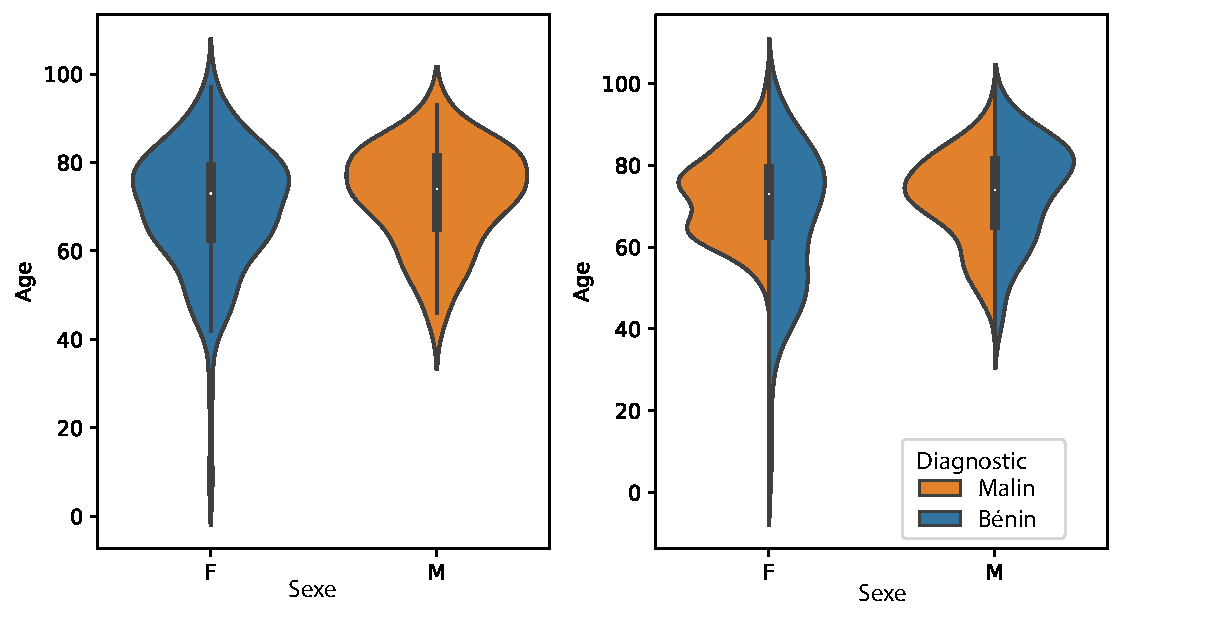
\includegraphics[width=0.8\linewidth]{contents/chapter_2/resources/statistics_age_sex.pdf}
    \caption{A gauche, répartition en fonction de l'âge et du sexe. A droite, répartition entre l'âge et le sexe en tenant compte du diagnostic binaire.}
    \label{fig:statistics}
\end{figure}\par

En ce qui concerne leur acquisition, celle-ci a été à chaque fois réalisée par l'un des 3 experts investigateurs de l'étude clinique~\cite{Cinotti2018}. Tout cas de collisions de tumeurs au sein d'un même groupe a été exclu de cette étude. En ce qui concerne la modalité de dermatoscopie, les données ont été produites à l'aide d'une caméra PowerShot® G7~\textsuperscript{\ref{footnote:device_powershot}} couplée au dispositif proposé par Fotofinder~\textsuperscript{\ref{footnote:device_fotofinder}}. Pour ce qui est de la modalité de \gls{rcm}, les données proviennent d'un VivaScope 3000®~\textsuperscript{\ref{footnote:device_mavig}}. En revanche, aucune information liée à l'acquisition des données de photographie clinique n'a été mentionnée.\par

L'intérêt de ces trois modalités est grand dans le contexte de la dermatologie puisqu'elles représentent le processus "classique" de prise en charge clinique, de la modalité la moins onéreuse avec la \textbf{photographie clinique} mais également la moins précise, à des modalités plus onéreuses, également plus riche en information, avec la \textbf{\gls{rcm}}. Ainsi, chaque modalité permet de réduire ainsi la zone d'incertitude chez un patient souffrant d'une pathologie de la peau.

\addtocounter{footnote}{1}
\footnotetext[\thefootnote]{Source : Canon Powershot®, Canon, Tokyo, Japon. \label{footnote:device_powershot}}
\addtocounter{footnote}{1}
\footnotetext[\thefootnote]{Source : FotoFinder Systems GmbH, Bad Birnbach, Allemagne. \label{footnote:device_fotofinder}}
\addtocounter{footnote}{1}
\footnotetext[\thefootnote]{Source : Distribué en Europe par MAVIG GmbH, Munich, Allemagne. \label{footnote:device_mavig}}

Afin d'évaluer les performances de praticiens face à ces lésions, les investigateurs ont eu recours à 21 dermatologues détenant une expertise des modalités d'imagerie non invasives. Ces experts sont répartis de manière homogène selon leurs compétences respectives pour chacun des dispositifs. Ainsi, le panel d'évaluation se décompose de la façon suivante: 
\begin{inlinerate}
\item 6 experts sont soumis à l'ensemble des modalités,
\item 15 experts sont soumis à l'évaluation de la photographie clinique et de la dermoscopie (dont 9 uniquement dédiés a ces deux modalités),
\item et 12 sont soumis à la \gls{rcm} (dont 6 uniquement dédiés à la \gls{rcm})~\cite{Cinotti2018}.
\end{inlinerate}
Cette répartition est résumée en \Cref{fig:experts_evaluation}. Pour chaque cas clinique étudié, ces experts ont évalué la gravité du cas à l'aide des termes bénin et malin.\par

\begin{figure}[H]
    \centering
    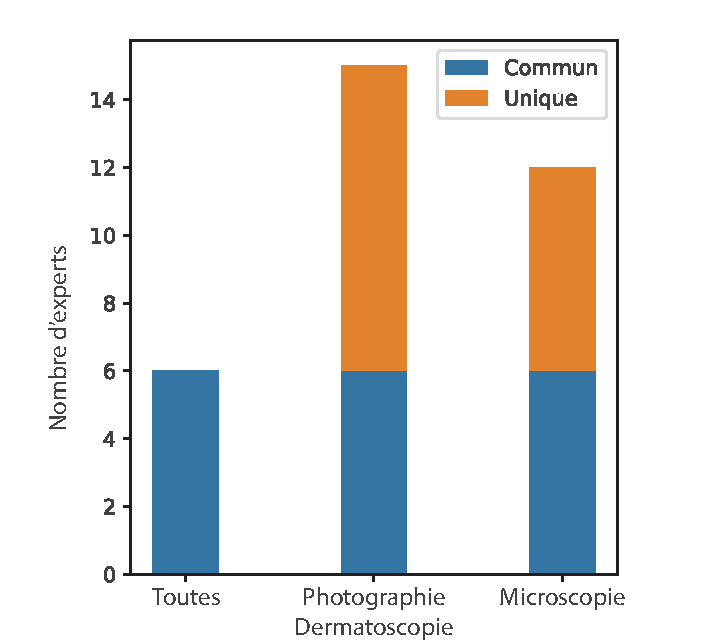
\includegraphics[width=0.6\linewidth]{contents/x_clinical_data/resources/experts_evaluation.pdf}
    \caption{Répartition du panel de 21 dermatologues sur l'évaluation des diverses modalités~\cite{Cinotti2018}.}
    \label{fig:experts_evaluation}
\end{figure}\par

Pour éviter tout biais dans l'évaluation, les experts évalués sur l'ensemble des modalités ont été sollicités sur trois journées différentes: 
\begin{inlinerate}
\item une première évaluation ne comprenant que les images de photographie clinique et de dermoscopie,
\item une seconde évaluation ne comprenant que les images de \gls{rcm}
\item et une dernière évaluation sur l'ensemble de la base d'images.
\end{inlinerate}
Par ailleurs, les cas cliniques ont été présentés dans un ordre différents entre chaque journée d'évaluation afin d'éviter des biais liés à l'activité précédente des experts.\par

% \subsection{Résultats des experts}

Afin de réaliser nos divers tests, une base d'images anonymisée nous a été remise, composée :
\begin{itemize}
\item d'un fichier tableau de lésions comprenant:
    \begin{inlinerate}
        \item en colonne, les diverses informations: \textit{Âge, Sexe,	Zone, Côté,	Diagnostic Binaire et Diagnostic},
        \item en ligne, les divers enregistrement liée à chaque lésion.
    \end{inlinerate}
    \item d'un répertoire comprenant les images des divers cas clinique recensés dans l'étude sous divers formats image.
\end{itemize}\par

Afin d'exploiter au mieux cette base, quelques modifications y sont apportées. D'une part, la diversité des formats images est un frein quand à la gestion de ces données et nous avons opté pour un format matriciel sans perte de type bitmap. D'autre part, la structure de la base ne permet pas l'utilisation d'annotation au niveau des images ou des instances autres. Afin de rendre plus dynamique cette partie, nous avons opté pour une structure reprenant le fichier table initial (au format \gls{csv}) et de répertoires associés à chaque lésion. Chaque dossier de lésion se compose lui même de fichiers d'annotation propre au type de données stockées (images ou patchs). Par ailleurs, certains apports d'informations ont été réalisés pour permettre un bon déroulement de la suite de notre travail, tel que l'appartenance à un patient. La \Cref{fig:db_structure} synthétise la structure de cette base avant et après modification.\par

\begin{figure}[H]
\centering
    \begin{subfigure}{.45\textwidth}
      \centering
      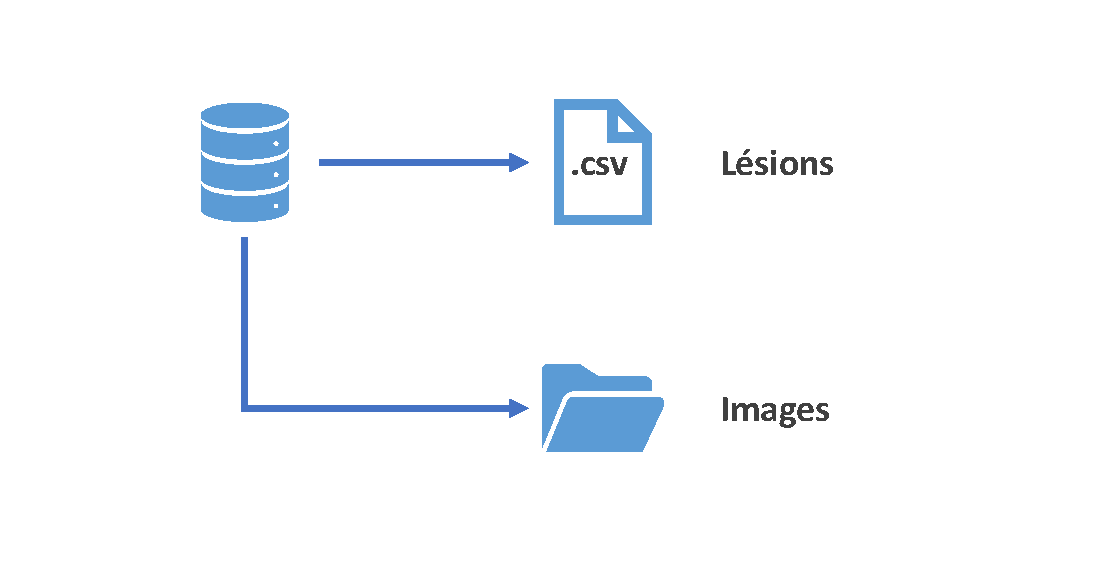
\includegraphics[width=\linewidth]{contents/x_clinical_data/resources/scheme_dbstructure_old.pdf}
    \end{subfigure}
    \begin{subfigure}{.45\textwidth}
      \centering
      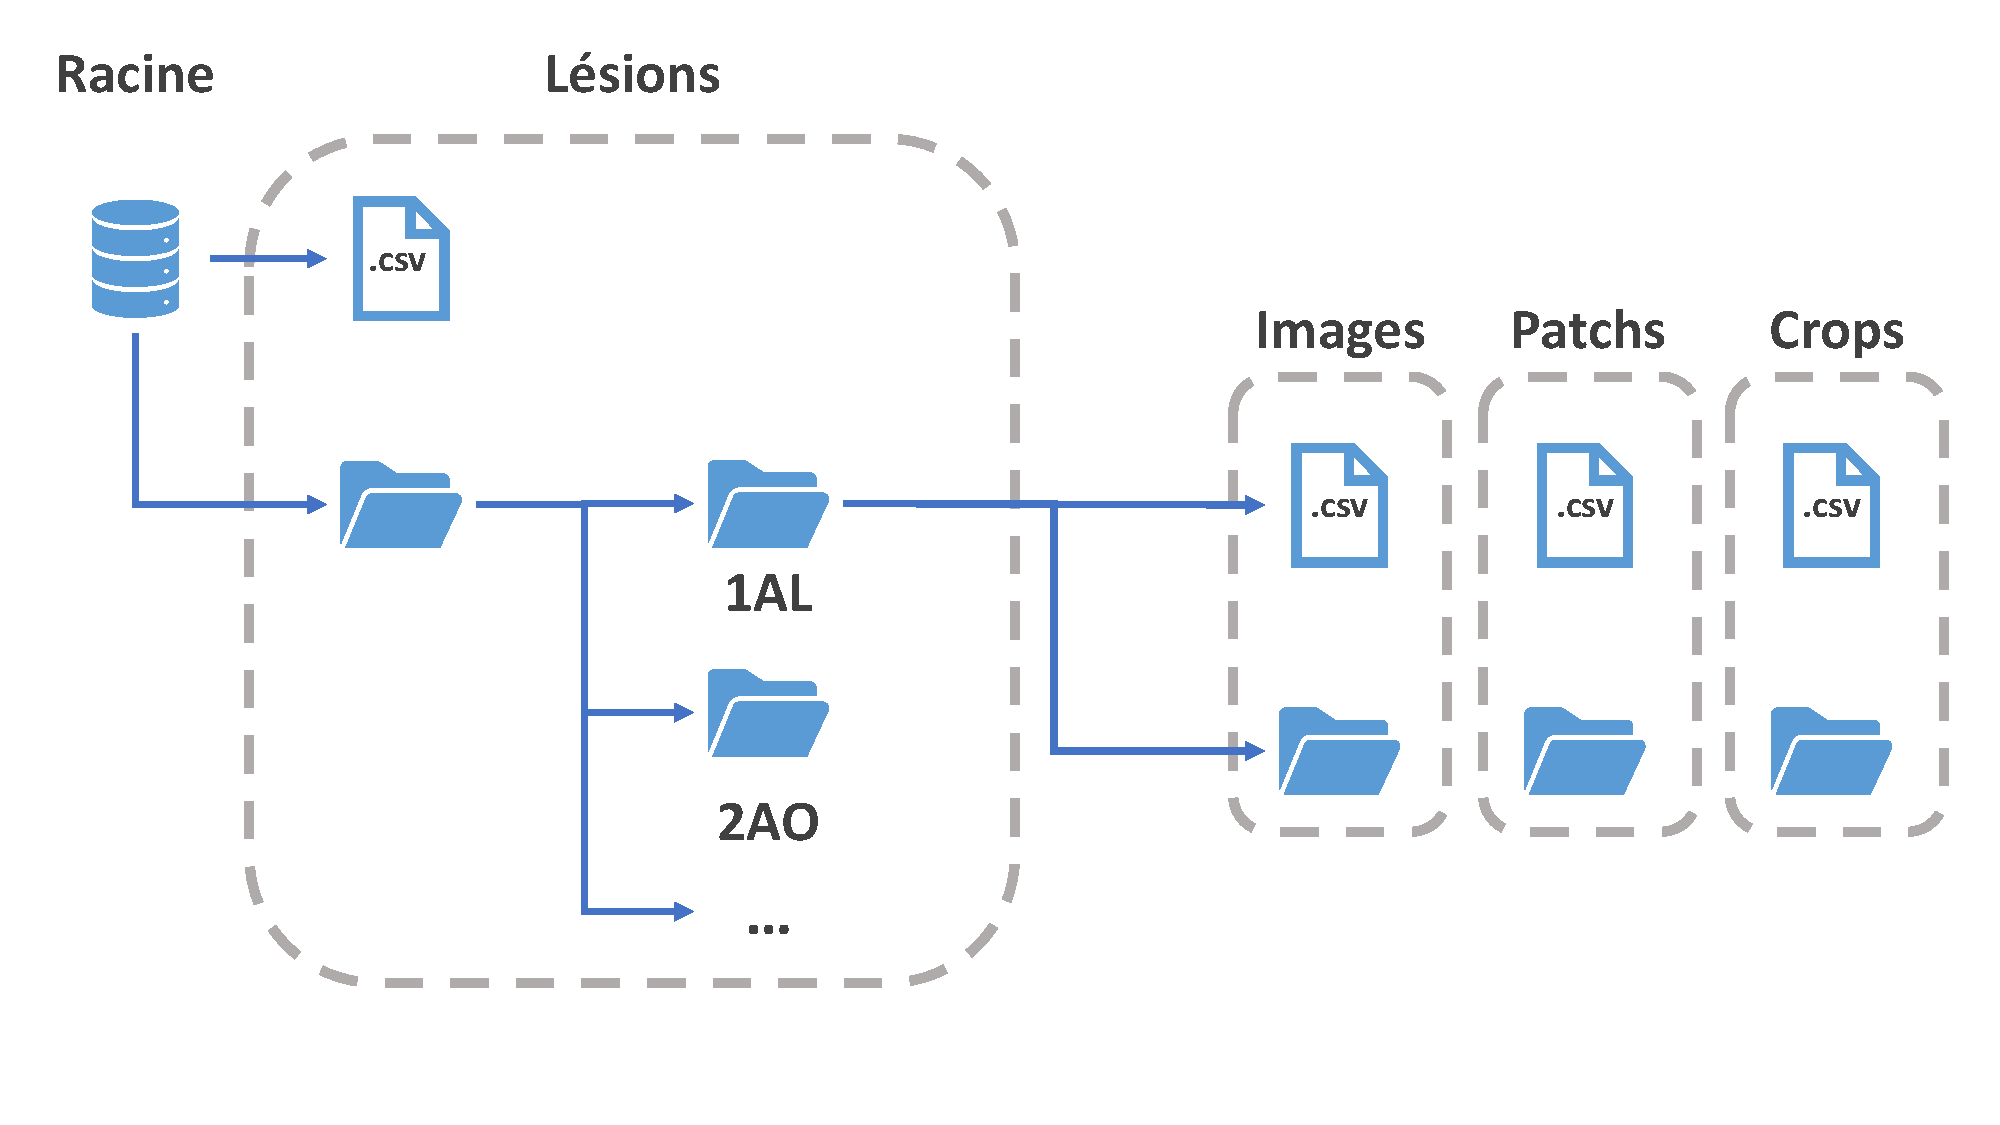
\includegraphics[width=\linewidth]{contents/x_clinical_data/resources/scheme_dbstructure_new.pdf}
    \end{subfigure}
    \caption{Schéma de l'organisation de la base de ressources employée. A gauche, la base initiale et à droite, la base restructurée afin de supporter de nouvelles annotations.}
    \label{fig:db_structure}
\end{figure}\par